% !Mode:: "TeX:UTF-8"
%此为第一章节。
%\figure为图片,[h]为hear代码所在,\caption为表名图名,\includegraphics为引用位置,\cite为引用参考文献,\begin{equation}公式,\subfloat子图,\label标签,\begin{table}表格,\begin{tabular}三线表,{cccc}完全居中,\toprule,\multirow取几行,\cmidrule取第几列\begin{theorem}定理,\begin{proof}证明,\begin{corollary}推论,\begin{lemma}引理
    
\chapter{绪\quad 论}
\section{课题的研究背景与意义}

\begin{shaded}
    微电子器件整体发展趋势  
    \end{shaded}
    与传统的二维图像信息相比,物体的三维信息能够更全面、真实的反映客观物体,为人们提供更多的信息量。通过三维测量得到物体空间坐标信息,并对这些数据进行分析处理后,其结果可以广泛应用于计算机辅助设计与制造(CAD/CAM)、反求工程(RE)、快速原型(RP)及虚拟现实(VR)等领域,具有较高的实用价值[1]。其中,三维信息的测量技术是基础,数据处理技术是核心,特征提取技术是关键,3个部分既相互补充又相互促进。

\subsection{三维测量与重构技术研究现状}
实体的三维测量与CAD模型的重构是反求工程的两个主要阶段,本节重点总结了与课题相关的基于层析数据的三维测量与实体重构技术的国内外研究现状。一、三维实体测量技术


    \begin{figure}[h]
        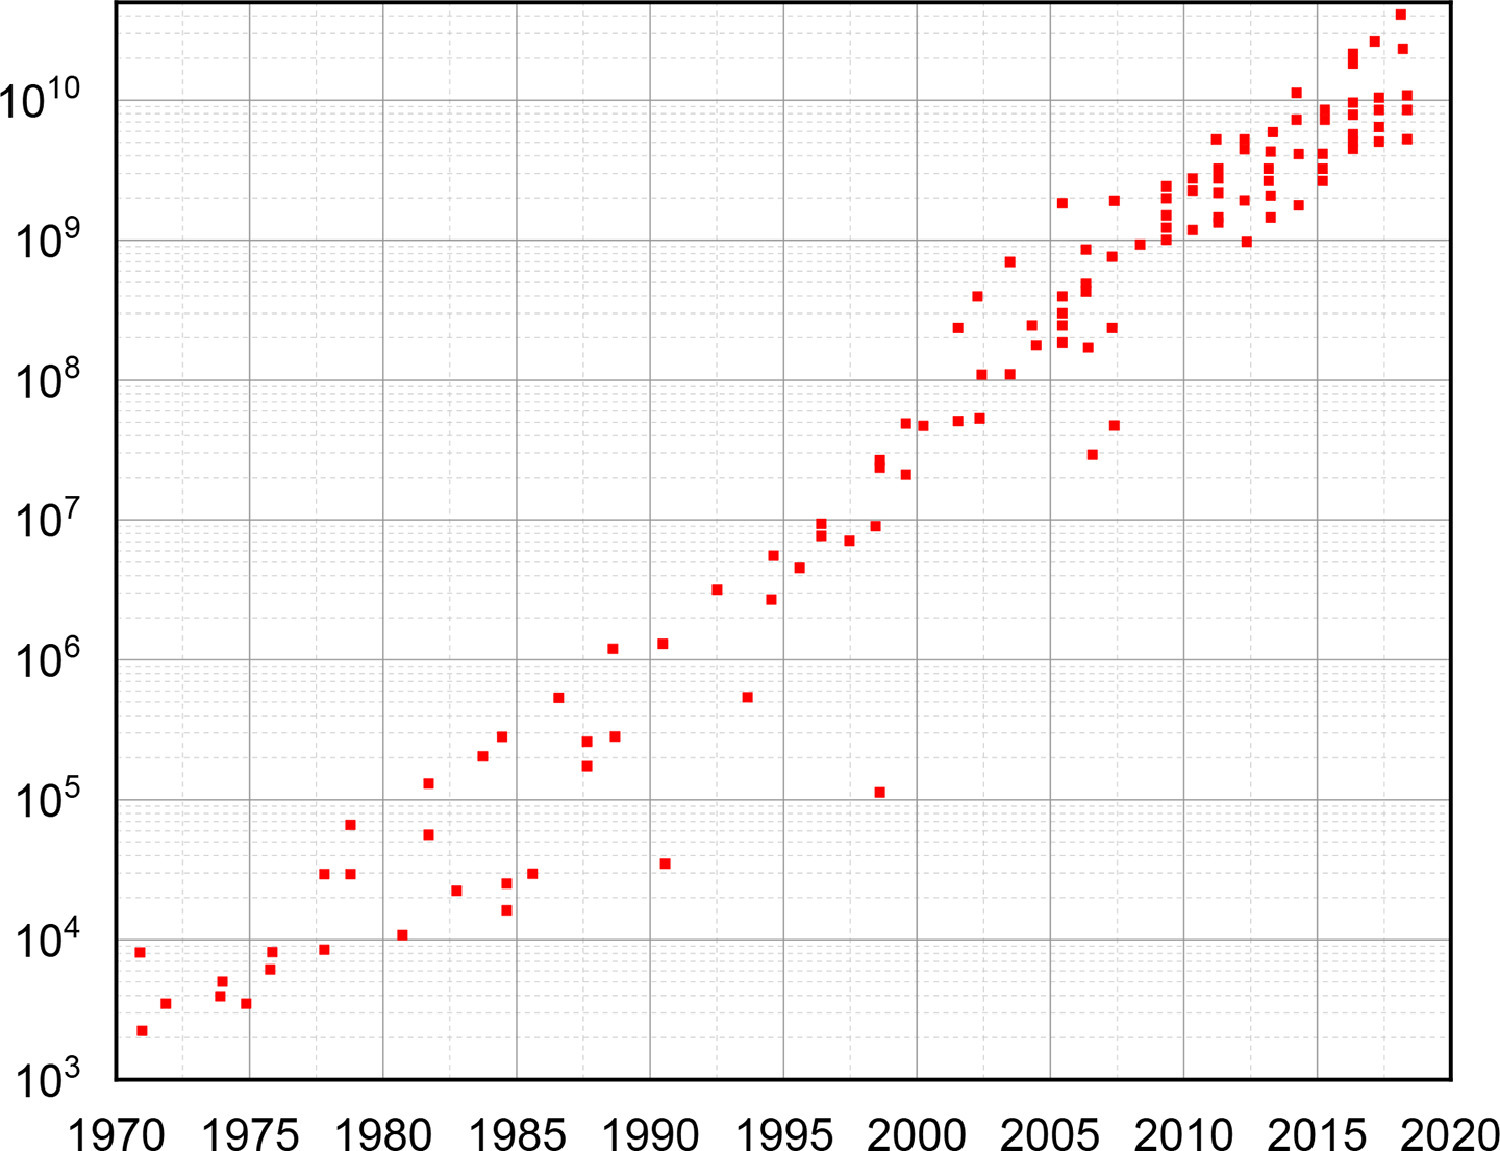
\includegraphics[width =0.5\linewidth]{chip-develop.jpg}
        \caption{半导体芯片上的晶体管数量}
        \label{chip-develop}
        \end{figure}


    \begin{equation}
        MTF = \frac{1}{{A{J^2}}}{\rm{exp}} - \frac{\phi }{{{K_B}T}}
        \label{MTF}
        \end{equation}



本论文以时域积分方程时间步进算法的数值实现技术、后时稳定性问题以及两层平面波加速算法为重点研究内容,主要创新点与贡献如下:

        \begin{algorithm}[H]
            \KwData{this text}
            \KwResult{how to write algorithm with \LaTeX2e}
            initialization\;
            \While{not at end of this document}{
                read current\;
                \eIf{understand}{
                    go to next section\;
                    current section becomes this one\;
                }{
                    go back to the beginning of current section\;
                }
            }
            \caption{How to wirte an algorithm.}
        \end{algorithm}

